\chapter{LBNF}
\label{ch:exec-summ-lbnf}


%%%%%%%%%%%%%%%%%%%%%%%%%%%%%%%%%%%%%%%%%%%%%%%%%%%%%%%%%%%%%%%%%%%%
\section{Introduction}
\label{sec:exec-summ-lbnf-intro}

\fixme{(0.5 pages, introduce idea of firing a neutrino beam 800 miles, from Fermilab to the far detector at Sanford Underground Research + near detector to sample unoscillated beam). Make conn beam spectrum needed for DUNE physics programme}
%%%%%%%%%%%%%%%%%%%%%%%%%%%%%%%%%%%%%%%%%%%%%%%%%%%%%%%%%%%%%%%%%%%%
\section{LBNF Neutrino Beam}
\label{sec:exec-summ-lbnf-bm}

\fixme{3 pg}

%%%%%%%%%%%%%%%%%%%%%%%%%%%%%%%%%%%%
\subsection{Fermilab Accelerator Complex and PIP-II}
\label{sec:exec-summ-lbnf-accel}

\fixme{figure}

%%%%%%%%%%%%%%%%%%%%%%%%%%%%%%%%%%%%
\subsection{Target, Horns and Decay tunnel}
\label{sec:exec-summ-lbnf-target}

\fixme{figure showing optimized target/horn configuration)}

%%%%%%%%%%%%%%%%%%%%%%%%%%%%%%%%%%%%
\subsection{Neutrino Beam Flux}
\label{sec:exec-summ-lbnf-flux}

\fixme{figure showing beam spectrum, details of neutrino flavour mix, some comments on uncertainties}

%%%%%%%%%%%%%%%%%%%%%%%%%%%%%%%%%%%%%%%%%%%%%%%%%%%%%%%%%%%%%%%%%%%%
\section{LBNF Conventional Facilities}
\label{sec:exec-summ-lbnf-cf}

\fixme{3 pg}

%%%%%%%%%%%%%%%%%%%%%%%%%%%%%%%%%%%%
\subsection{Near Detector Facility at Fermilab}
\label{sec:exec-summ-lbnf-cf-near}

\fixme{1 page, figure?, some general information, location, depth, distance from target, etc.)}

%%%%%%%%%%%%%%%%%%%%%%%%%%%%%%%%%%%%
\subsection{Far Detector Facility at SURF}
\label{sec:exec-summ-lbnf-cf-far}

\fixme{2 pages, figure, description of caverns, chambers, central utility, strategic motivation for 4 chambers}

%%%%%%%%%%%%%%%%%%%%%%%%%%%%%%%%%%%%%%%%%%%%%%%%%%%%%%%%%%%%%%%%%%%%
\section{Far Detector Cryostats and Cryogenics Infrastructure}
\label{sec:exec-summ-lbnf-cryo}

%%%%%%%%%%%%%%%%%%%%%%%%%%%%%%%%%%%%
\subsection{Cryostats}
\label{sec:exec-summ-lbnf-cryostats}


%%%%%%%%%%%%%%%%%%%%%%%%%%%%%%%%%%%%
\subsection{Cryogenics Infrastructure}
\label{sec:exec-summ-lbnf-cryogen}

%%%%%%%%%%%%%%%%%%%%
\subsubsection{Internal Cryogenics}
\label{sec:exec-summ-lbnf-int-cryogen}
% from David 2/8/2018

The LBNF internal cryogenics system consists of a set of pipes and manifolds that distribute liquid and gaseous argon (LAr and GAr) inside each LBNF cryostat. The components are: 
\fixme{are there pipes that are not part of the manifolds? Clarify distinction between manifolds and pipes}


\begin{itemize}
\item a dedicated GAr-purge manifold located just above the floor of the cryostat; currently this manifold consists of seven pipes running over the floor under the detector, \SI{1360}{mm} from each other;
\fixme{``currently?'' need number for final design!}
\item dedicated LAr-GAr mist feedthroughs, distributed along the long dimension of the cryostat roof, ten on each side, outside the detector zone;
\item a LAr distribution manifold located on the floor of the cryostat; and
\item additional distribution manifolds with calibrated holes or slits in the pipes;
these manifolds connect to the cryostat through the top plate via dedicated feedthroughs.
\end{itemize}

The piping is illustrated in Figures~\ref{fig:cryo-internal-piping-3D} and~\ref{fig:cryo-internal-piping-2D}.
\begin{dunefigure}[optional caption for LoF]{fig:cryo-internal-piping-3D}
     {Provide full caption (Credit: xyz?)}
    %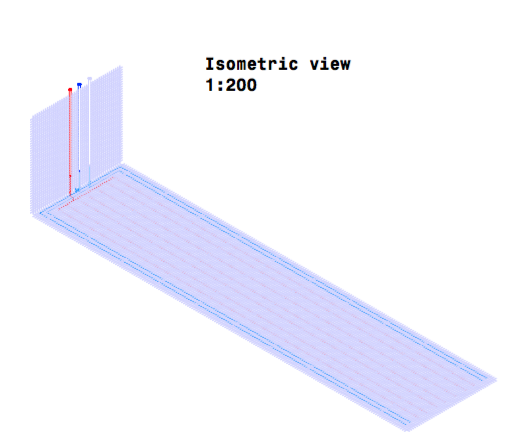
\includegraphics[width=0.5\textwidth]{cryo-internal-piping-3D}
\end{dunefigure}

\begin{dunefigure}[optional caption for LoF]{fig:cryo-internal-piping-2D}
     {Provide full caption (Credit: xyz?)}
    %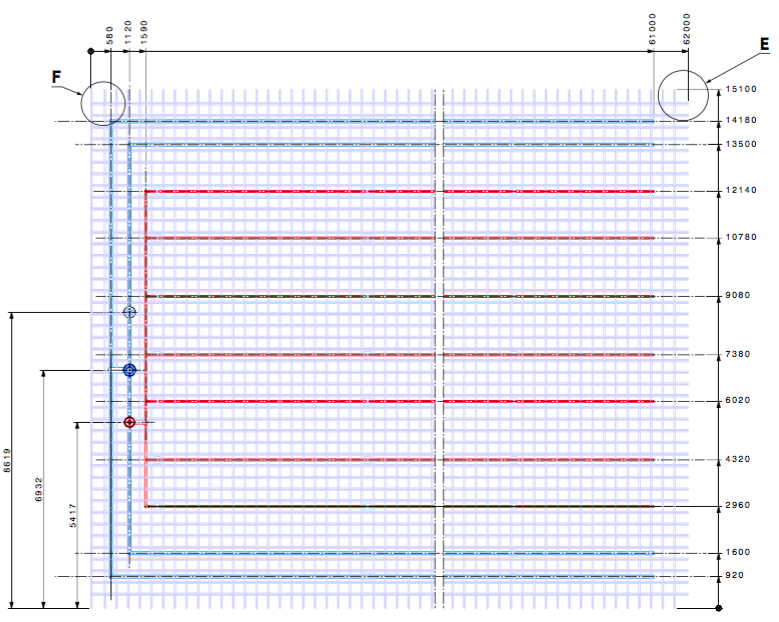
\includegraphics[width=0.7\textwidth]{cryo-internal-piping-2D}
\end{dunefigure}

This system supports the following operations:

\begin{itemize}
\item Initial GAr purge. This purge removes impurities and lowers the contaminants (oxygen and water) to the parts per million (ppm) or sub-ppm range. The dedicated GAr-purge manifold distributes the GAr uniformly using either calibrated holes or a longitudinal slit along the length of the pipes. 
\fixme{is the decision not made, or are both holes and slit in the design?}

\item Cryostat cool-down. Once the impurities are removed, a mist of liquid and gaseous argon cools the cryostat and detector to the desired temperature before the LAr fill commences. The LAr-GAr mist is injected through dedicated feedthroughs, each with two nozzles. The mixing nozzle generates a LAr-GAr mist with a flat profile. The second nozzle sprays GAr only; this spray moves the mist around inside the cryostat to achieve a uniform cooling.

\item Cryostat fill. Once the cryostat and detector are cold, the filling can commence. GAr is transferred from the surface to the 4850L underground where condensers located on the mezzanine above the cryostat recondense it. LAr flows from the condensers into the cryostat where it is released using the LAr distribution manifold. Two \fixme{additional?} manifolds distribute the LAr through four pipes, two per manifold, located along the long sides of the cryostat, outside the detector footprint. Calibrated holes along the pipes guarantee a uniform distribution of the liquid.

\item Normal operations. During normal operations, the purge manifold and cool-down feedthroughs are not in service. LAr is continuously recirculated and returned to the cryostat via the LAr distribution manifold.
\end{itemize}

The design parameters for the first cryostat are listed in Table~\ref{tab:lbnf-int-cryogen-param}. The design temperature and pressure for all pipes will be \SI{77}{K} and \SI{100}{psig}.

\begin{dunetable}
[Internal cryogenics system parameters, first cryostat]
{lr}
{tab:lbnf-int-cryogen-param}
{Internal cryogenics system parameters, first cryostat}
  Parameter & Flow rate \\ \toprowrule
  Piston Purge Flow rate (From 1.2 m/hr GAr linear motion) & \SI{1123}{m$^3$/hr} \\ \colhline
 Maximum cool-down rate of TPC & \SI{40}{K/hr} (\SI{10}{K/m}) \\ \colhline
  Maximum {$\Delta$}T between any two points of the detector & \SI{50}{K}  \\ \colhline
  Desired cool-down rate of detector and membrane & \num{10}-\SI{15}{K/hr}  \\ \colhline
  Fill flow rate (from current schedule) & \SI{0.8}{kg/s} \\ \colhline
%  \makecell[l]{LAr purification flow rate to achieve purity \\ (four LAr pumps running)} & \SI{36}{kg/s} \\ \colhline
%  \makecell[l]{LAr purification flow rate during normal operations \\ (one pump running in continuous operation)}
% Anne writes: makecell works in pdflatex but not overleaf.
  LAr purification flow rate to achieve purity \\ (four LAr pumps running) & \SI{36}{kg/s} \\ \colhline
  LAr purification flow rate during normal operations \\ (one pump running in continuous operation)
 & \SI{9}{kg/s}\\
\end{dunetable}
